\documentclass[12pt, spanish]{article}
\usepackage[spanish]{babel}
\selectlanguage{spanish}
%\usepackage{natbib}
\usepackage{url}
\usepackage[utf8x]{inputenc}
\usepackage{graphicx}
\graphicspath{{images/}}
\usepackage{parskip}
\usepackage{fancyhdr}
\usepackage{vmargin}
\usepackage{multirow}
\usepackage{float}
\usepackage{chngpage}

\usepackage{amsfonts}

\usepackage{subcaption}

\usepackage{hyperref}
\usepackage[
    type={CC},
    modifier={by-nc-sa},
    version={4.0},
]{doclicense}

\hypersetup{
    colorlinks=true,
    linkcolor=blue,
    filecolor=magenta,
    urlcolor=cyan,
}

% para codigo
\usepackage{listings}
\usepackage{xcolor}



%% configuración de listings

\definecolor{listing-background}{HTML}{F7F7F7}
\definecolor{listing-rule}{HTML}{B3B2B3}
\definecolor{listing-numbers}{HTML}{B3B2B3}
\definecolor{listing-text-color}{HTML}{000000}
\definecolor{listing-keyword}{HTML}{435489}
\definecolor{listing-identifier}{HTML}{435489}
\definecolor{listing-string}{HTML}{00999A}
\definecolor{listing-comment}{HTML}{8E8E8E}
\definecolor{listing-javadoc-comment}{HTML}{006CA9}

\lstdefinestyle{eisvogel_listing_style}{
  language         = python,
%$if(listings-disable-line-numbers)$
%  xleftmargin      = 0.6em,
%  framexleftmargin = 0.4em,
%$else$
  numbers          = left,
  xleftmargin      = 0em,
 framexleftmargin = 0em,
%$endif$
  backgroundcolor  = \color{listing-background},
  basicstyle       = \color{listing-text-color}\small\ttfamily{}\linespread{1.15}, % print whole listing small
  breaklines       = true,
  frame            = single,
  framesep         = 0.19em,
  rulecolor        = \color{listing-rule},
  frameround       = ffff,
  tabsize          = 4,
  numberstyle      = \color{listing-numbers},
  aboveskip        = 1.0em,
  belowskip        = 0.1em,
  abovecaptionskip = 0em,
  belowcaptionskip = 1.0em,
  keywordstyle     = \color{listing-keyword}\bfseries,
  classoffset      = 0,
  sensitive        = true,
  identifierstyle  = \color{listing-identifier},
  commentstyle     = \color{listing-comment},
  morecomment      = [s][\color{listing-javadoc-comment}]{/**}{*/},
  stringstyle      = \color{listing-string},
  showstringspaces = false,
  escapeinside     = {/*@}{@*/}, % Allow LaTeX inside these special comments
  literate         =
  {á}{{\'a}}1 {é}{{\'e}}1 {í}{{\'i}}1 {ó}{{\'o}}1 {ú}{{\'u}}1
  {Á}{{\'A}}1 {É}{{\'E}}1 {Í}{{\'I}}1 {Ó}{{\'O}}1 {Ú}{{\'U}}1
  {à}{{\`a}}1 {è}{{\'e}}1 {ì}{{\`i}}1 {ò}{{\`o}}1 {ù}{{\`u}}1
  {À}{{\`A}}1 {È}{{\'E}}1 {Ì}{{\`I}}1 {Ò}{{\`O}}1 {Ù}{{\`U}}1
  {ä}{{\"a}}1 {ë}{{\"e}}1 {ï}{{\"i}}1 {ö}{{\"o}}1 {ü}{{\"u}}1
  {Ä}{{\"A}}1 {Ë}{{\"E}}1 {Ï}{{\"I}}1 {Ö}{{\"O}}1 {Ü}{{\"U}}1
  {â}{{\^a}}1 {ê}{{\^e}}1 {î}{{\^i}}1 {ô}{{\^o}}1 {û}{{\^u}}1
  {Â}{{\^A}}1 {Ê}{{\^E}}1 {Î}{{\^I}}1 {Ô}{{\^O}}1 {Û}{{\^U}}1
  {œ}{{\oe}}1 {Œ}{{\OE}}1 {æ}{{\ae}}1 {Æ}{{\AE}}1 {ß}{{\ss}}1
  {ç}{{\c c}}1 {Ç}{{\c C}}1 {ø}{{\o}}1 {å}{{\r a}}1 {Å}{{\r A}}1
  {€}{{\EUR}}1 {£}{{\pounds}}1 {«}{{\guillemotleft}}1
  {»}{{\guillemotright}}1 {ñ}{{\~n}}1 {Ñ}{{\~N}}1 {¿}{{?`}}1
  {…}{{\ldots}}1 {≥}{{>=}}1 {≤}{{<=}}1 {„}{{\glqq}}1 {“}{{\grqq}}1
  {”}{{''}}1
}
\lstset{style=eisvogel_listing_style}


\usepackage[default]{sourcesanspro}

\setmarginsrb{2 cm}{1 cm}{2 cm}{2 cm}{1 cm}{1.5 cm}{1 cm}{1.5 cm}

\title{Práctica 1:\\
Diferentes modelos de simulación.\hspace{0.05cm} }
\author{Antonio David Villegas Yeguas}
\date{\today}

\renewcommand*\contentsname{hola}

\makeatletter
\let\thetitle\@title
\let\theauthor\@author
\let\thedate\@date
\makeatother

\pagestyle{fancy}
\fancyhf{}
\rhead{\theauthor}
\lhead{\thetitle}
\cfoot{\thepage}

\begin{document}

%%%%%%%%%%%%%%%%%%%%%%%%%%%%%%%%%%%%%%%%%%%%%%%%%%%%%%%%%%%%%%%%%%%%%%%%%%%%%%%%%%%%%%%%%

\begin{titlepage}
    \centering
    \vspace*{0.3 cm}
    
\includegraphics[scale = 0.50]{ugr.png}\\[0.7 cm]
    %\textsc{\LARGE Universidad de Granada}\\[2.0 cm]
    \textsc{\large 4º CSI 2020/21 - Grupo 1}\\[0.5 cm]
    \textsc{\large Grado en Ingeniería Informática}\\[0.5 cm]
    \rule{\linewidth}{0.2 mm} \\[0.2 cm]
    { \huge \bfseries \thetitle}\\
    \rule{\linewidth}{0.2 mm} \\[1 cm]

    \begin{minipage}{0.4\textwidth}
        \begin{flushleft} \large
            \emph{Autor:}\\
            \theauthor\\
			 \emph{DNI:}\\
            77021623-M
            \end{flushleft}
            \end{minipage}~
            \begin{minipage}{0.4\textwidth}
            \begin{flushright} \large
            \emph{Asignatura: \\
            Simulación de Sistemas}   \\
            \emph{Correo:}\\
            advy99@correo.ugr.es
        \end{flushright}
    \end{minipage}\\[0.5cm]

    {\large \thedate}\\[0.5cm]
    %{\url{https://github.com/advy99/AA/}}
    {\doclicenseThis}

    \vfill

\end{titlepage}

%%%%%%%%%%%%%%%%%%%%%%%%%%%%%%%%%%%%%%%%%%%%%%%%%%%%%%%%%%%%%%%%%%%%%%%%%%%%%%%%%%%%%%%%%

\tableofcontents
\pagebreak

%%%%%%%%%%%%%%%%%%%%%%%%%%%%%%%%%%%%%%%%%%%%%%%%%%%%%%%%%%%%%%%%%%%%%%%%%%%%%%%%%%%%%%%%%


\section*{Introducción}

En esta primera práctica se nos ha dado tres problemas distintos que debemos resolver mediante simulación. Se nos ha proporcionado un fichero en C++ para cada uno de estos problemas, que simula el sistema que queremos estudiar. Este PDF se encuentra el estudio sobre los distintos sistemas, así como ciertos experimentos de como se comportarían cada sistema si modificamos su funcionamiento, haciendo posible resolver cierto problema sobre estos sistemas sin tener que resolver el problema de forma analítica.

Los distintos sistemas tratan sobre:

\begin{enumerate}
	\item Modelo de simulación de Monte Carlo: Aparcamiento más cercano a un objetivo.
	\item Modelo de simulación discreto: Funcionamiento de radares.
	\item Modelo de simulación continuo: Lago con dos especies de peces.
\end{enumerate}


\section{Modelo de simulación de Monte Carlo.}

En este caso se nos plantea estudiar un sistema que simula el comportamiento de un conductor buscando aparcamiento. Como nos dice el enunciado, existen dos tipos de conductores, los que aparcan en el primer sitio libre que encuentran, y los que intentan aparcar en el destino. Nuestro programa de simulación simulará miles de veces un conductor que en un punto C decide aparcar en el primer sitio que encuentre, C tomará valores entre 0 (conductor que aparca en el primer sitio libre), hasta la posición de destino (conductor que intenta aparcar en el propio destino), de esta forma podremos estimar que tactica es mejor, y donde está el mejor punto para aparcar.

\subsection{Prueba del sistema con los parámetros por defecto.}

Para un primer análisis utilizaremos los valores dadas por defecto, 100000 simulaciones para evaluar la media, y cada simulación tendrá como destino el punto 100, el conductor tendrá una visión de 2 aparcamientos delante de él y la probabilidad de que un aparcamiento esté libre es del 90\%.

Tras varias ejecuciones vemos que la distancia mínima está al comenzar a buscar aparcamiento sobre la posición 94.

\begin{figure}[H]
	\centering
	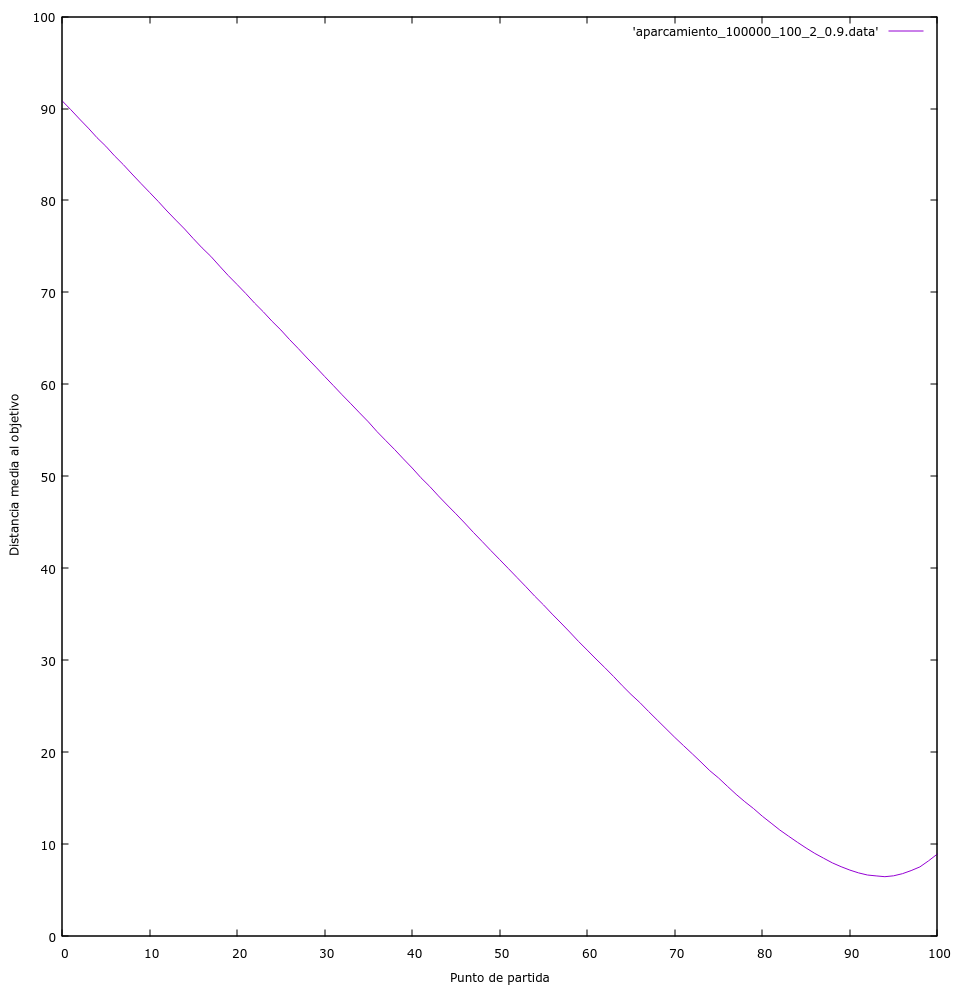
\includegraphics[scale = 0.6]{aparcamiento_100000_100_2_0-9.png}
	\caption{Distancia media al objetivo respecto al punto de partida.}
	\label{fig:ej4}

\end{figure}

Aunque vemos que la mejor posición para comenzar a buscar aparcamiento está sobre la posición 94, si observamos la desviación típica de esas medias vemos como el mínimo está en 85, con una desviación de 5.5 aproximadamente, mientras que la desviación típica más alta es de 9.6 aproximadamente, y en concreto en el mínimo que hemos encontrado, en el punto 94, de 7.42, por lo que podemos concluir que el mejor punto para comenzar a buscar aparcamiento es entre el 90 y 94, ya que cerca del 90 la media de distancia es más alta, sin embargo la desviación típica es menos, por lo que la media nos da valores más fiables, aunque en el puesto 94 nos de el mejor valor medio es posible que en ocasiones el el valor haya sido muy distinto (para bien o para mal) de dicha media.


\begin{figure}[H]
	\centering
	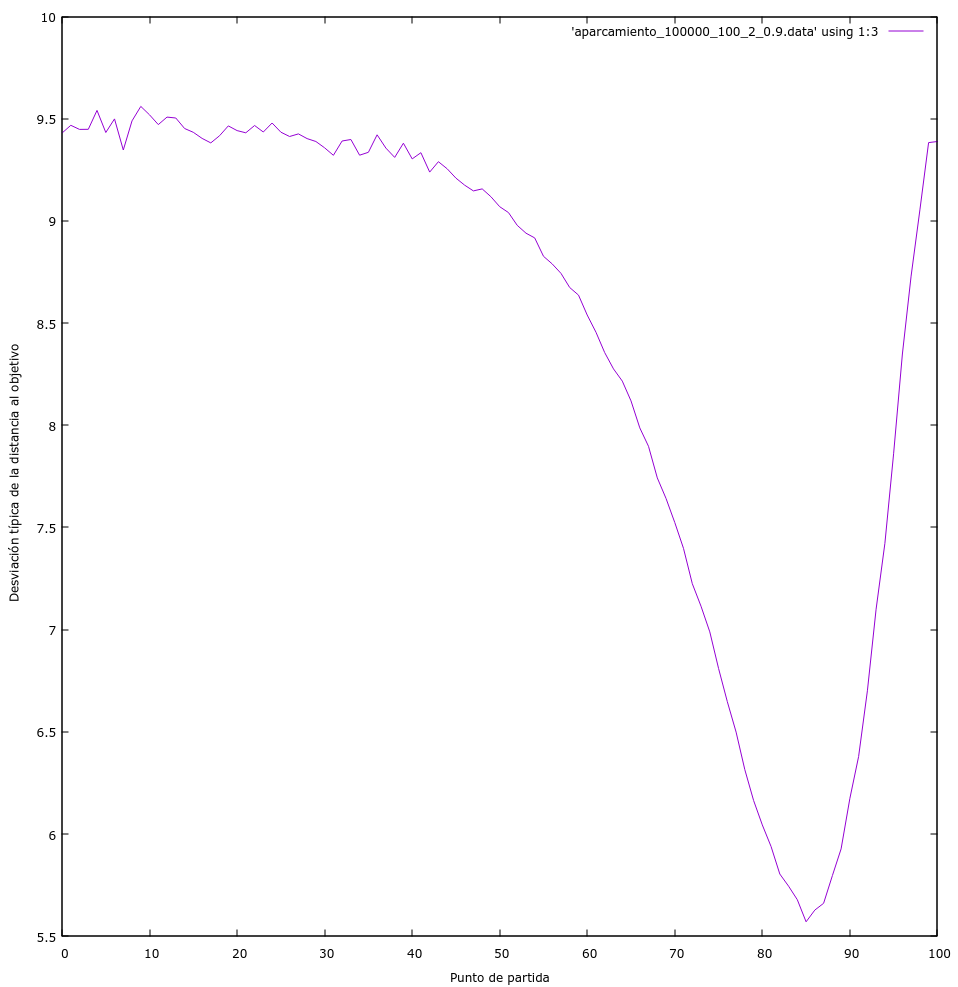
\includegraphics[scale = 0.6]{aparcamiento_desv_100000_100_2_0-9.png}
	\caption{Desviación típica de la media de la distancia al objetivo respecto al punto de partida.}
	\label{fig:ej4}
\end{figure}

\subsection{Variación de la posición destino.}

En este experimento simularemos el sistema modificando la posición del destino, ya que en el apartado anterior tal vez la posición inicial era tan pequeña que por este motivo las posiciones iniciales.


Tras realizar la prueba con valores de destino 125, 150, 175 y 200, además del objetivo inicial en 100, obtenemos los siguientes resultados:


\begin{figure}[H]
	\centering
	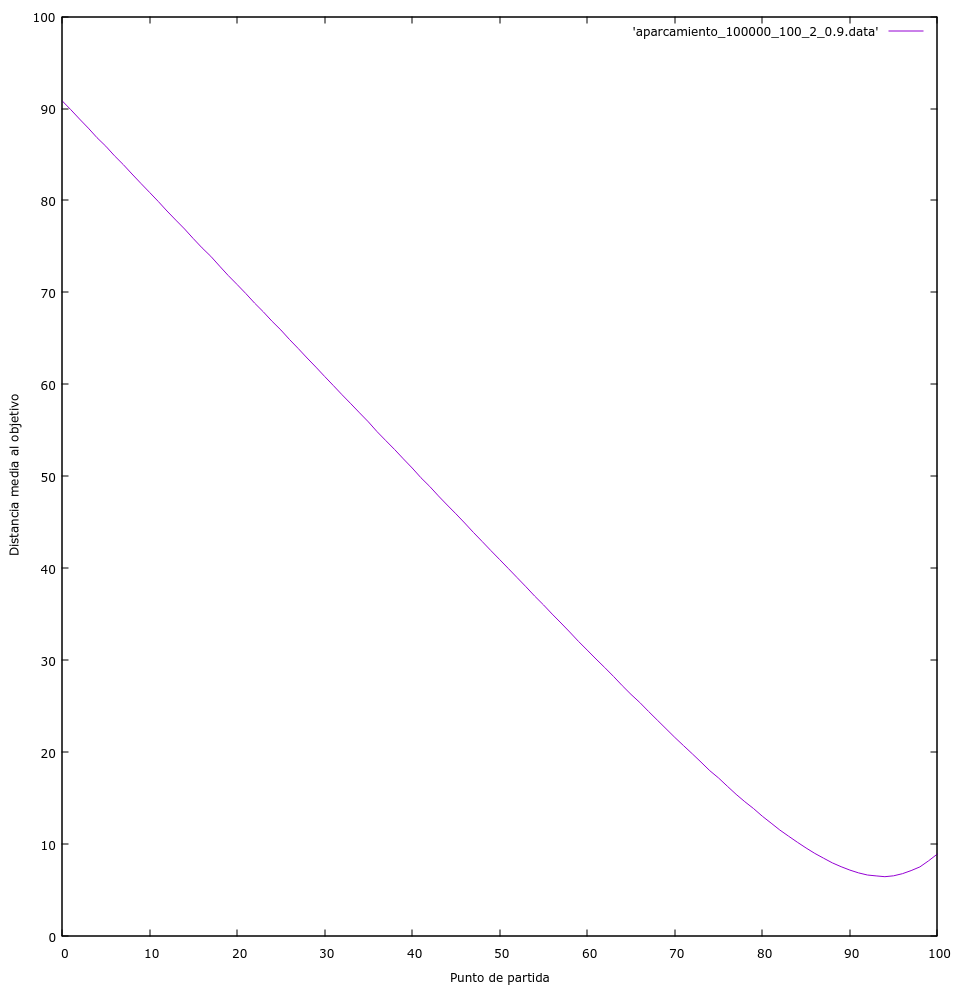
\includegraphics[scale = 0.6]{aparcamiento_100000_100_2_0-9.png}
	\caption{Media de la distancia al objetivo en 100 respecto al punto de partida.}
	\label{fig:ej4}
\end{figure}

\begin{figure}[H]
	\centering
	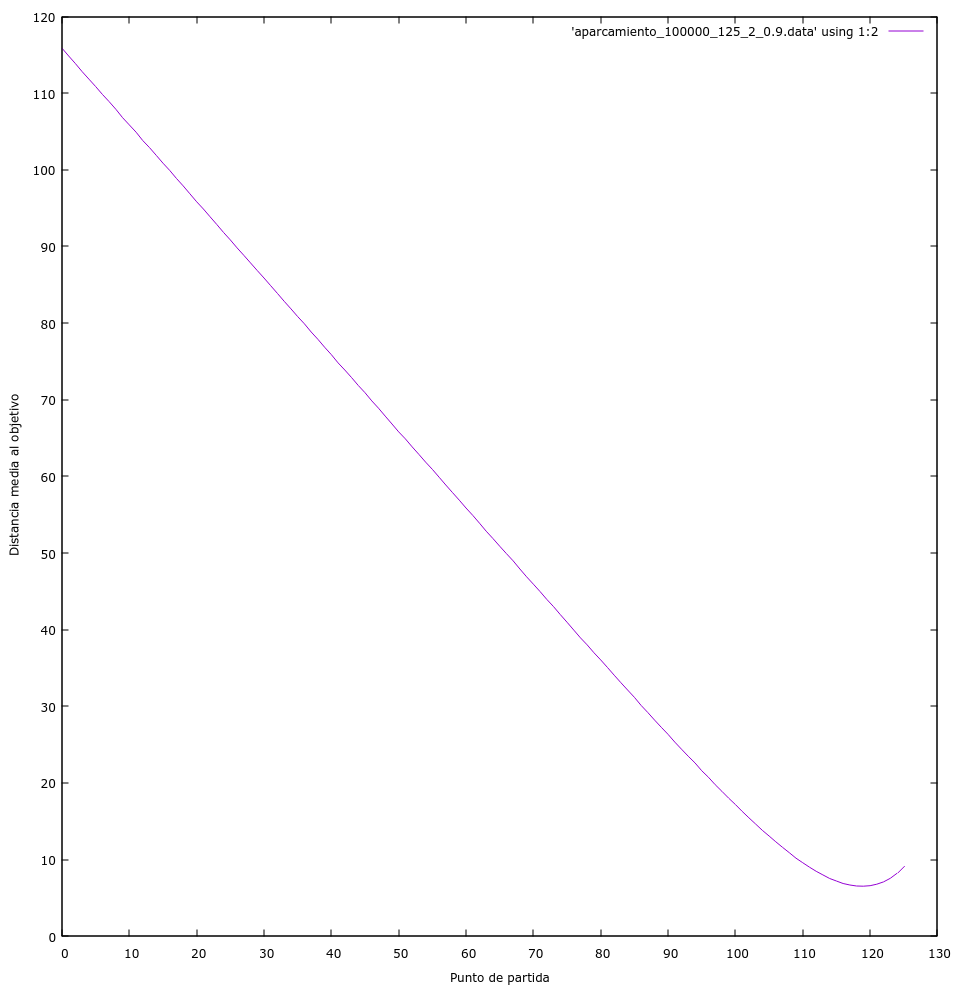
\includegraphics[scale = 0.6]{aparcamiento_100000_125_2_0-9.png}
	\caption{Media de la distancia al objetivo en 125 respecto al punto de partida.}
	\label{fig:ej4}
\end{figure}

\begin{figure}[H]
	\centering
	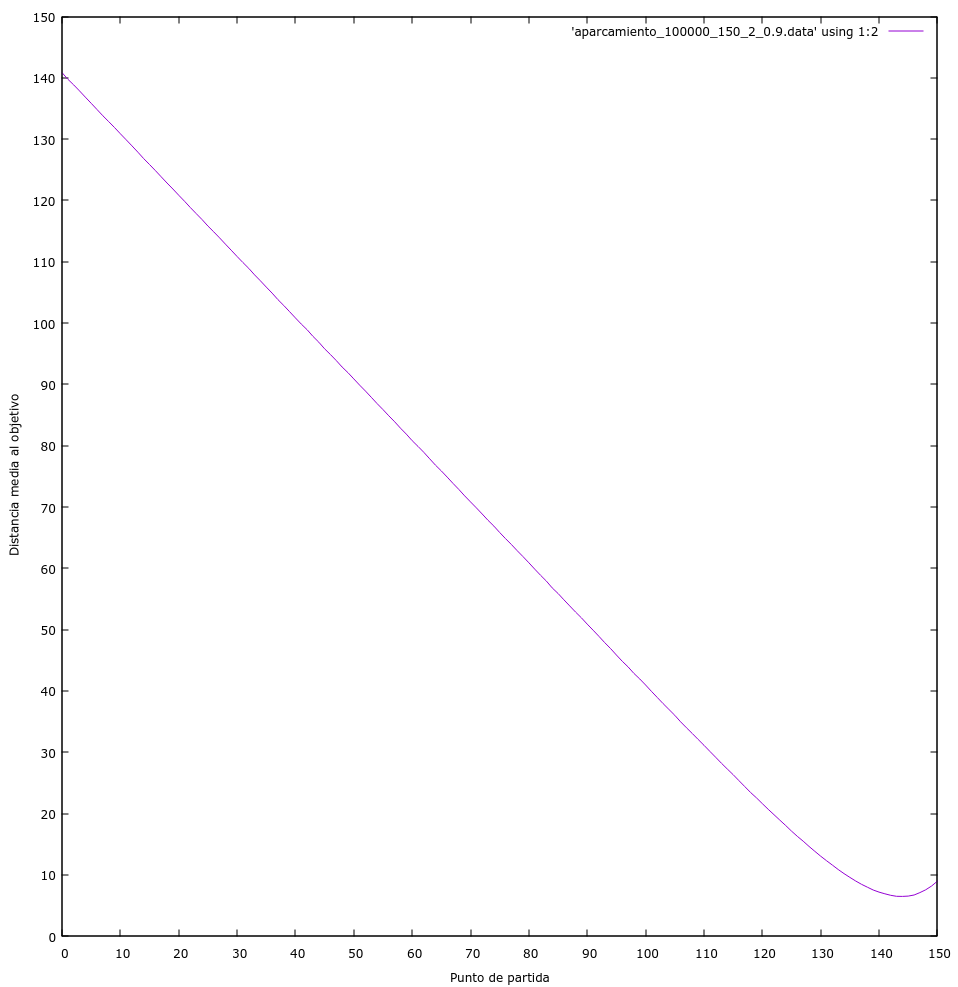
\includegraphics[scale = 0.6]{aparcamiento_100000_150_2_0-9.png}
	\caption{Media de la distancia al objetivo en 150 respecto al punto de partida.}
	\label{fig:ej4}
\end{figure}

\begin{figure}[H]
	\centering
	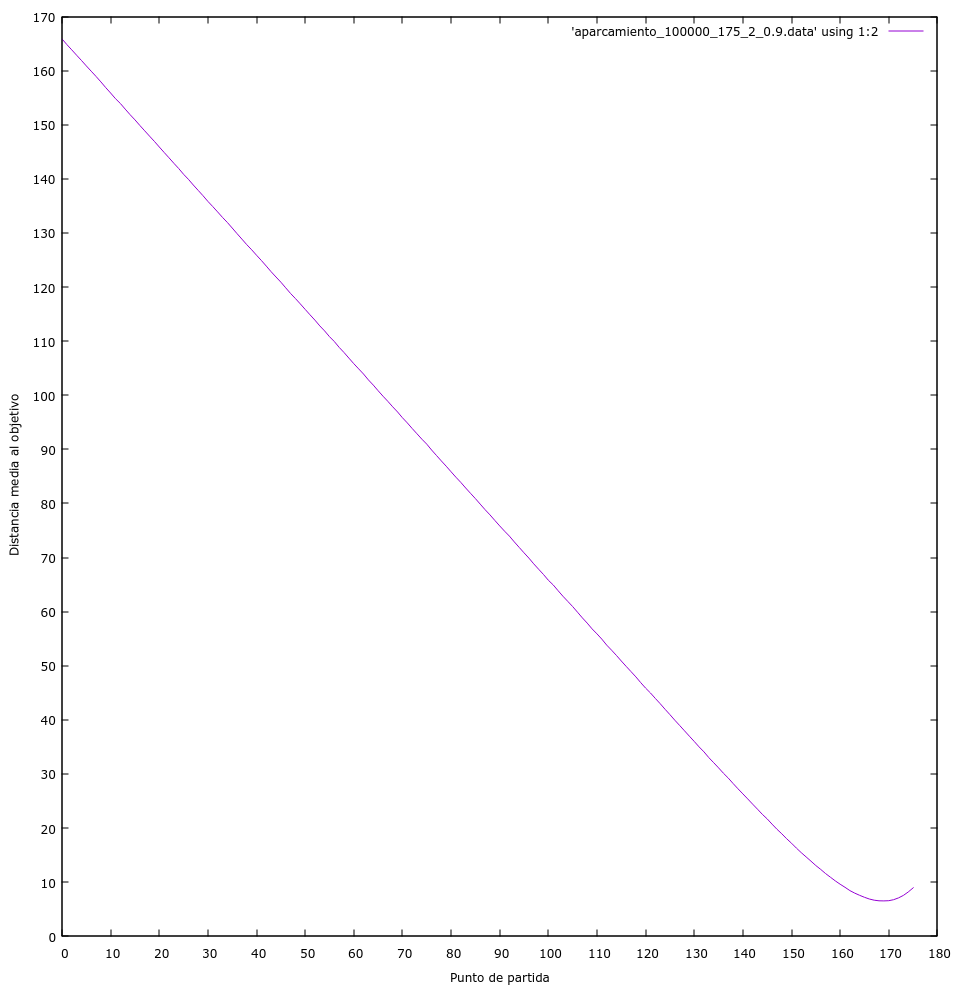
\includegraphics[scale = 0.6]{aparcamiento_100000_175_2_0-9.png}
	\caption{Media de la distancia al objetivo en 175 respecto al punto de partida.}
	\label{fig:ej4}
\end{figure}

\begin{figure}[H]
	\centering
	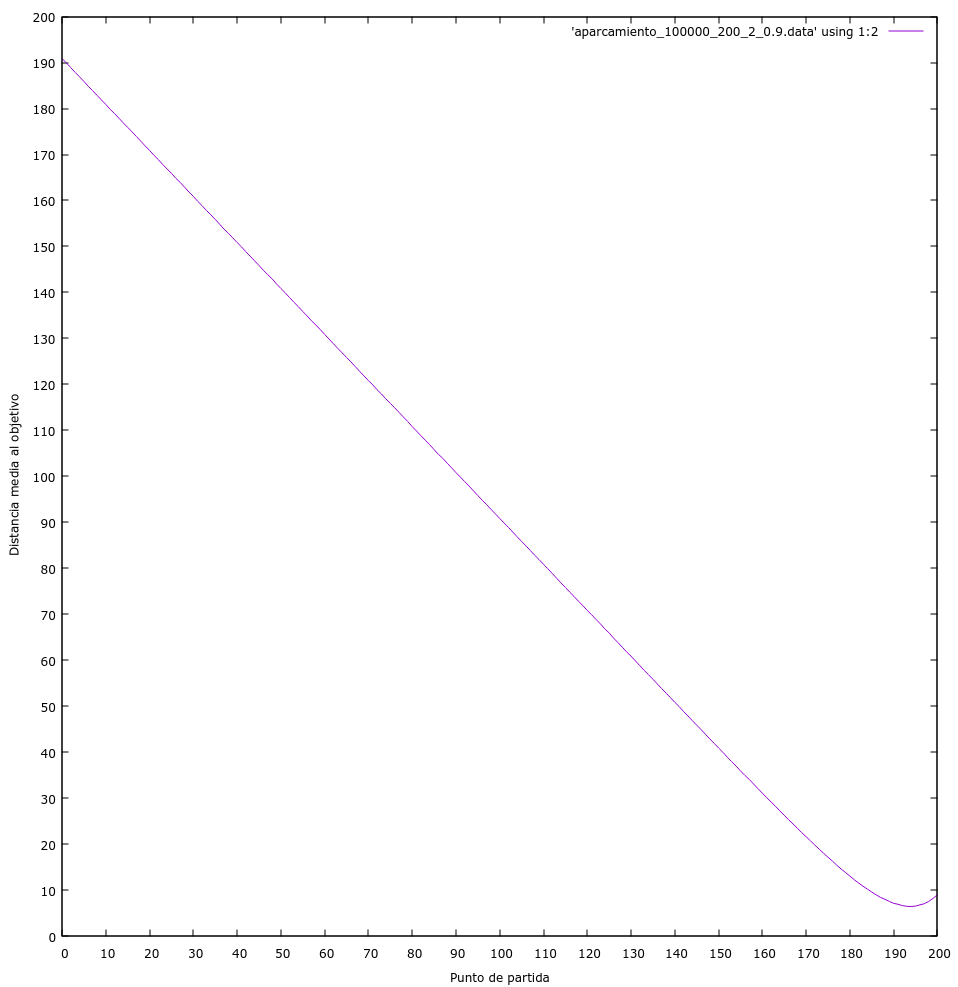
\includegraphics[scale = 0.6]{aparcamiento_100000_200_2_0-9.png}
	\caption{Media de la distancia al objetivo en 200 respecto al punto de partida.}
	\label{fig:ej4}
\end{figure}

Vemos como en todos los casos el óptimo se encuentra en unas 6-7 posiciones antes del objetivo, luego con este experimento podríamos llegar a concluir que el mejor punto para comenzar a buscar aparcamiento, con los parámetros fijos que utilizamos, es a unas 6-7 posiciones del objetivo.



\newpage

\subsection{Variación de la probabilidad de que un sitio este ocupado.}

En este caso probaré con distintos valores, entre ellos valores extremos para comprobar que el sistema se comporta de forma correcta. Probaré con 0.01, es decir, que la probabilidad de que esté ocupado es prácticamente nula, 0.25, 0.75 y por último y como caso extremo, 0.99, donde será muy dificil encontrar un sitio.

Tras lanzar las simulaciones obtenemos las siguientes gráficas:


\begin{figure}[H]
	\centering
	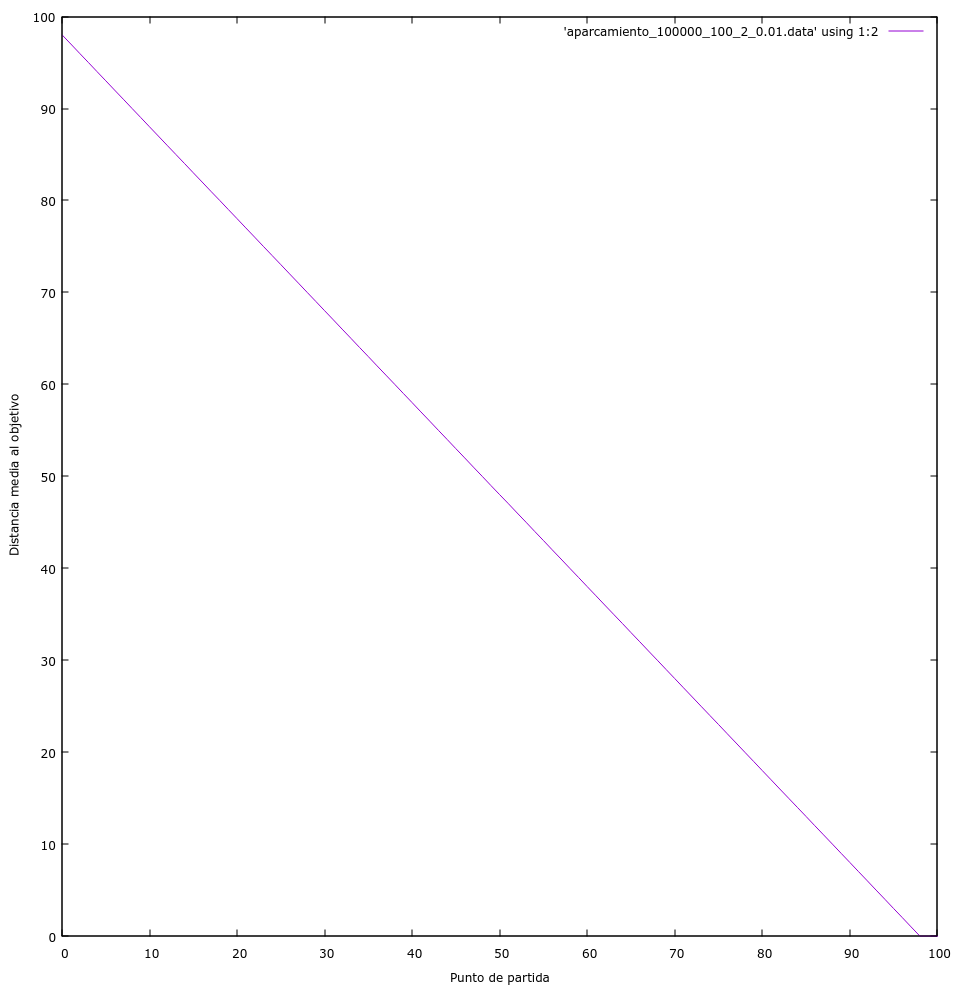
\includegraphics[scale = 0.6]{aparcamiento_100000_100_2_0-01.png}
	\caption{Media de la distancia al objetivo respecto al punto de partida con una probabilidad del 1\% de que el sitio este ocupado.}
	\label{fig:ej4}
\end{figure}

\begin{figure}[H]
	\centering
	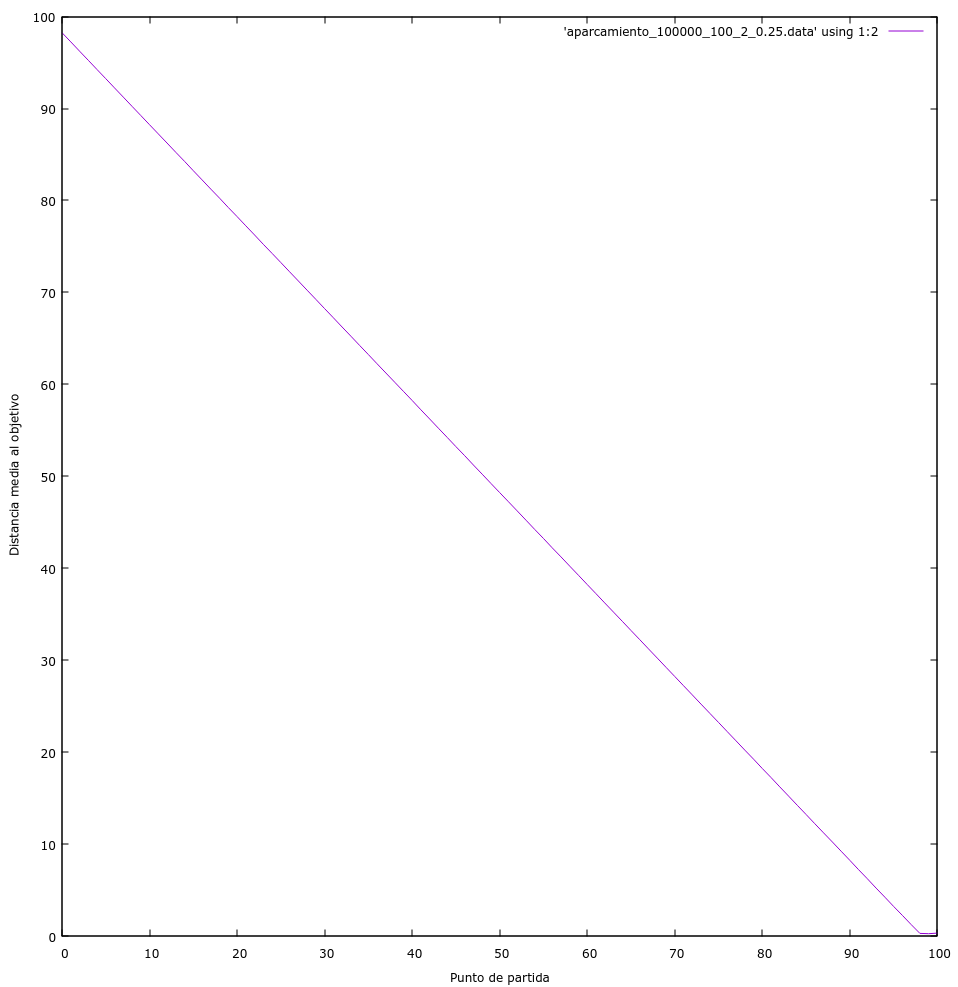
\includegraphics[scale = 0.6]{aparcamiento_100000_100_2_0-25.png}
	\caption{Media de la distancia al objetivo respecto al punto de partida con una probabilidad del 25\% de que el sitio este ocupado..}
	\label{fig:ej4}
\end{figure}

\begin{figure}[H]
	\centering
	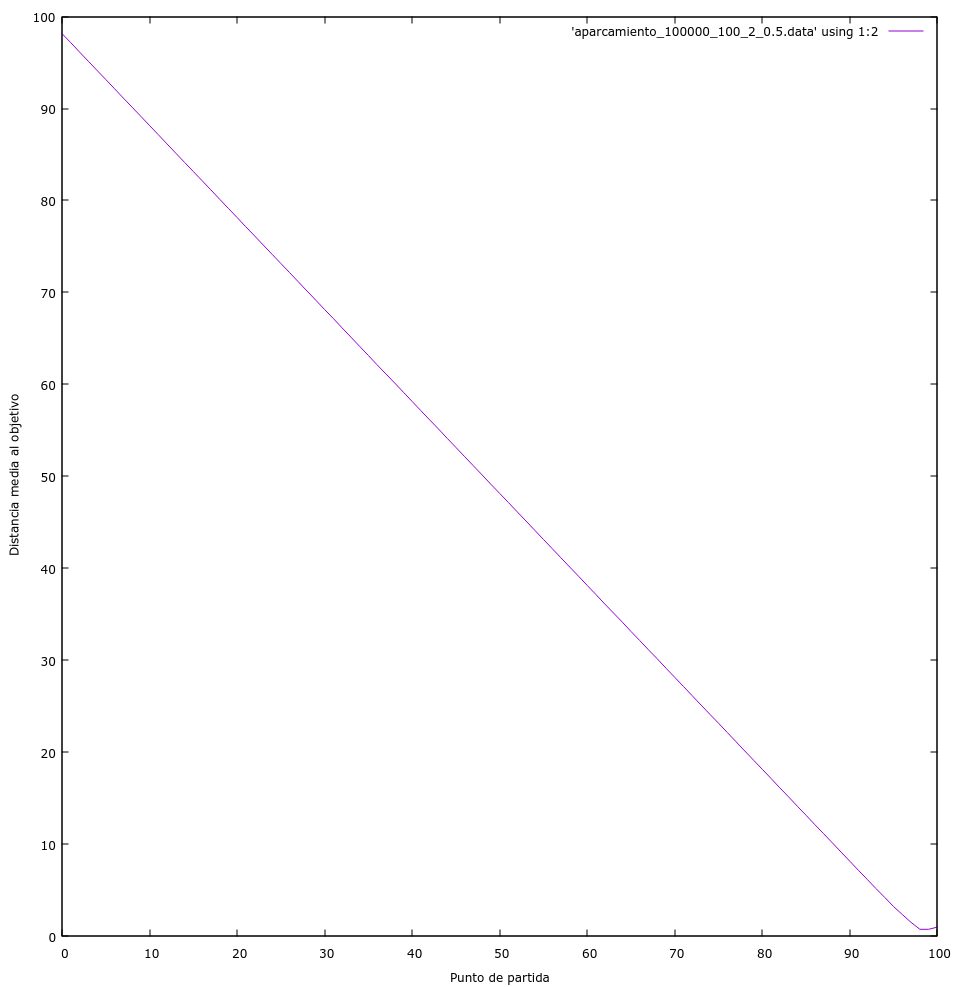
\includegraphics[scale = 0.6]{aparcamiento_100000_100_2_0-50.png}
	\caption{Media de la distancia al objetivo respecto al punto de partida con una probabilidad del 50\% de que el sitio este ocupado.}
	\label{fig:ej4}
\end{figure}

\begin{figure}[H]
	\centering
	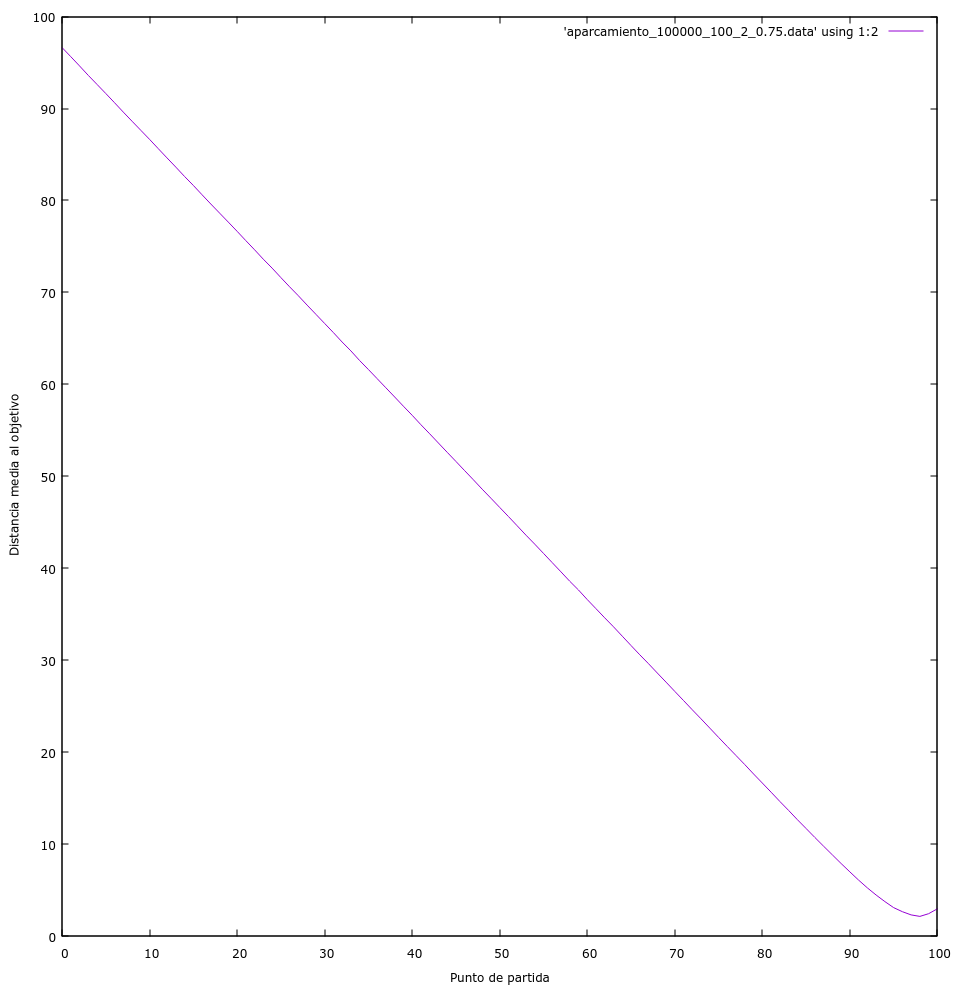
\includegraphics[scale = 0.6]{aparcamiento_100000_100_2_0-75.png}
	\caption{Media de la distancia al objetivo respecto al punto de partida con una probabilidad del 75\% de que el sitio este ocupado..}
	\label{fig:ej4}
\end{figure}

\begin{figure}[H]
	\centering
	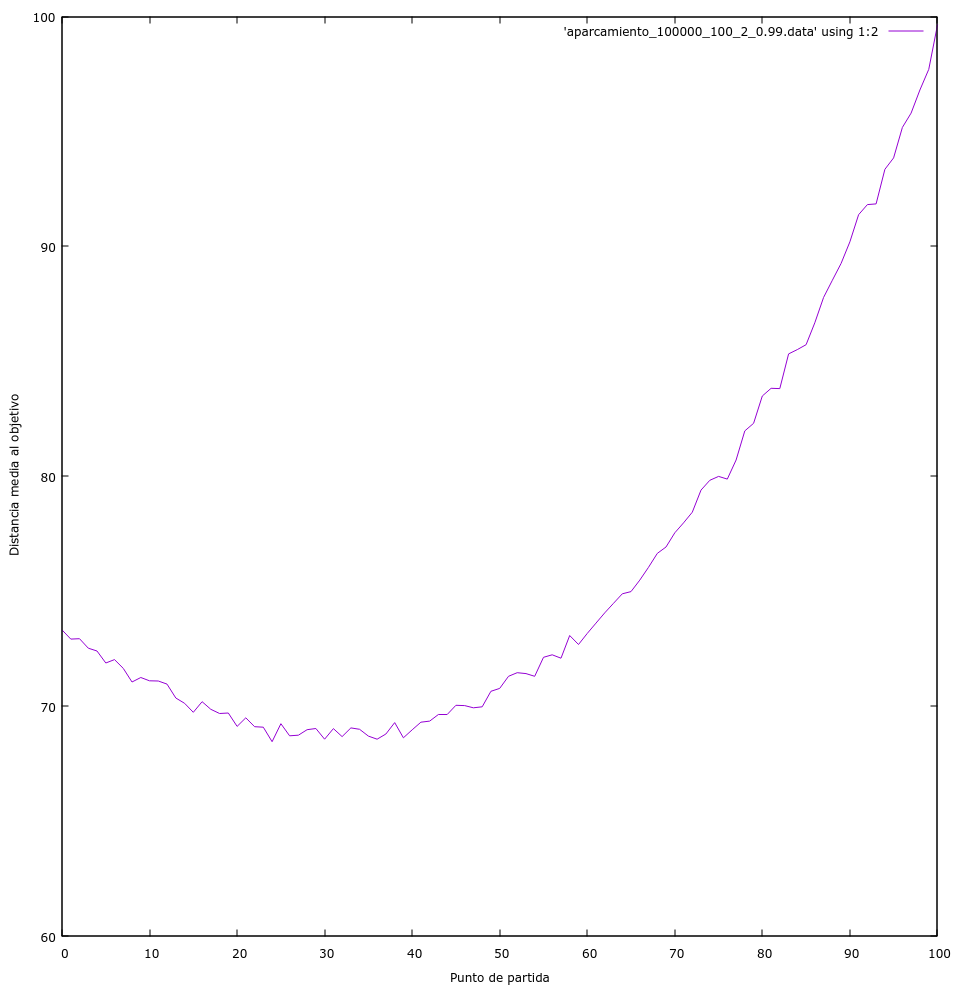
\includegraphics[scale = 0.6]{aparcamiento_100000_100_2_0-99.png}
	\caption{Media de la distancia al objetivo respecto al punto de partida con una probabilidad del 99\% de que el sitio este ocupado.}
	\label{fig:ej4}
\end{figure}


En este caso vemos como los casos extremos se comportan como esperabamos, en el caso de que un sitio esta ocupado con probabilidad 1\% podemos aparcar en la puerta con distancia 0, ya que es muy facil encontrar sitio, a medida que subimos el porcentaje se va haciendo más dificil encontrar sitio en el objetivo y comienza a ser buena idea comenzar a buscar sitio un poco antes de llegar, como habíamos visto en apartados anteriores, llegando al caso extremo en el que un sitio esta ocupado con una probabilidad del 99\%, que observamos que la menor distancia la obtenemos al comenzar a buscar apartamiento al principio. Este caso, al ser extremo, voy a estudiarlo también con la desviación típica de la media.


\begin{figure}[H]
	\centering
	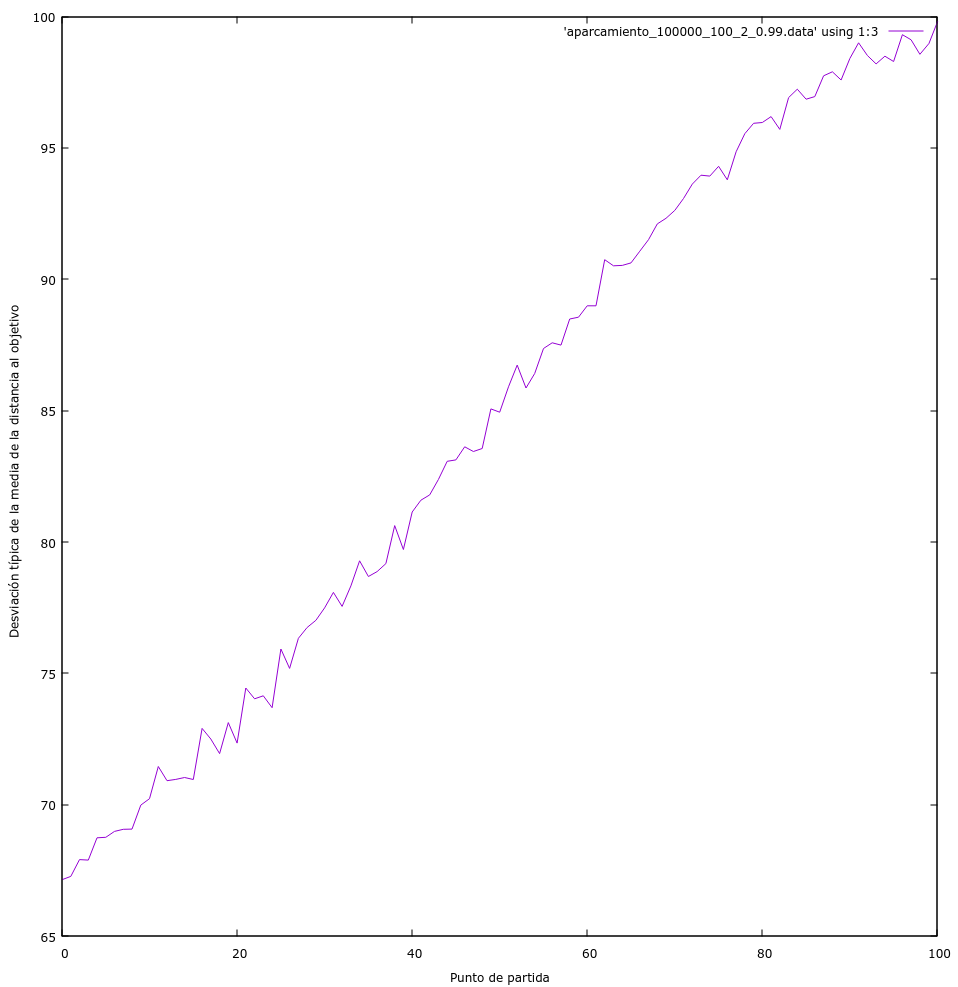
\includegraphics[scale = 0.6]{aparcamiento_desv_100000_100_2_0-99.png}
	\caption{Desv. típica de la media de la distancia al objetivo respecto al punto de partida con una probabilidad del 99\% de que el sitio este ocupado.}
	\label{fig:ej4}
\end{figure}


Observamos que para este caso el resultado es apenas fiable, ya que la desviación típica es del orden de la propia distancia máxima a recorrer, de entre 70 a 90 de distancia, mientras que en los casos menos extremos, como por ejemplo una probabilidad de ocupación del 90\% nos encontrabamos con una desviación típica de entre 5 y 9.

Este resultado sigue teniendo sentido en nuestro sistema, ya que la probabilidad de encontrar sitio es tan baja, que prácticamente es imposible llegar a un buen resultado comenzando a buscar aparcamiento cerca del objetivo, de ahí que la mejor opción sea encontrar desde el comienzo.

\subsection{Modificando la distancia de visión y la probabilidad de que el sitio esté ocupado}

En este caso, para intentar ver como interaccionan estos dos valores, he realizado la simulación modificando los parámetros, obteniendo la siguiente gráfica.

\begin{figure}[H]
	\centering
	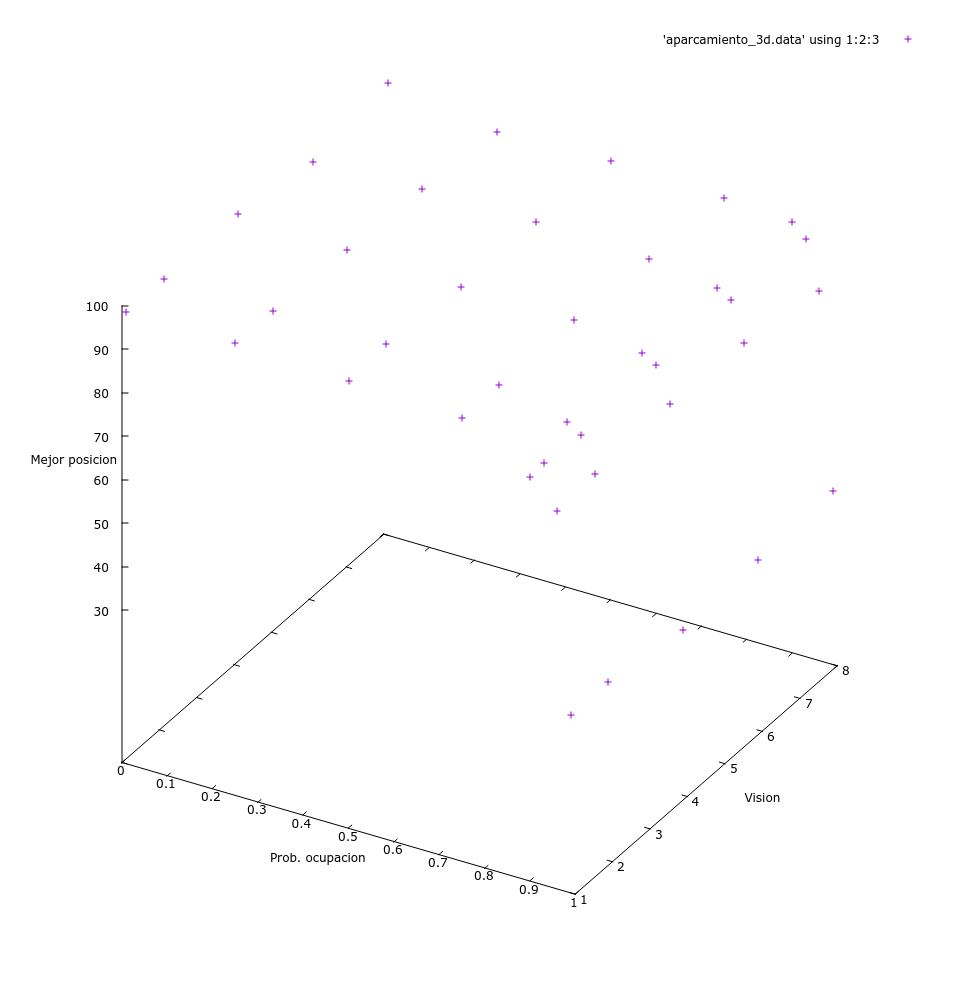
\includegraphics[scale = 0.55]{aparcamiento_3d.png}
	\caption{Media de la distancia al objetivo respecto al punto de partida con distintas probabilidades de ocupación y visión del conductor.}
	\label{fig:ej4}
\end{figure}

Vemos que como esperabamos, con baja probabilidad la mejor posición es 100, y que con respecto aumentamos esa probabilidad la mejor posición cada vez está más alejada del objetivo, y también podemos observar que si mejoramos la distancia de visión del conductor esa posición también se va acercando al objetivo, aunque no es un factor tan importante como la probabilidad de que un sitio esté ocupado.


\section{Modelo de simulación discreto.}

El sistema a estudiar en este caso trata sobre el funcionamiento de ciertos radares, que cuentan con cierto componente que falla de forma periódica. Se nos pide estudiar el sistema para saber el número mínimo de repuestos, con un número fijo de radares, sabiendo que cada vez que una de estas piezas se rompe, tarda un cierto tiempo en ser reparada, y su repuesto es demasiado caro, haciendo que queramos tener el mínimo número de repuestos, pero siempre y cuando no exista un periodo en el que un radar este sin funcionar.

\subsection{Estudio del funcionamiento con distintos tiempos de simulación.}

En este apartado trataremos de encontrar el número mínimo de repuestos para los parámetros por defecto, 5 radares, con un tiempo de vida de aproximadamente 20 días y en los que cada pieza tarda en repararse entre 15 y 30 días.

Tras realizar varias ejecuciones con distintos tiempos de simulación obtenemos los siguientes resultados:


\begin{figure}[H]
	\centering
	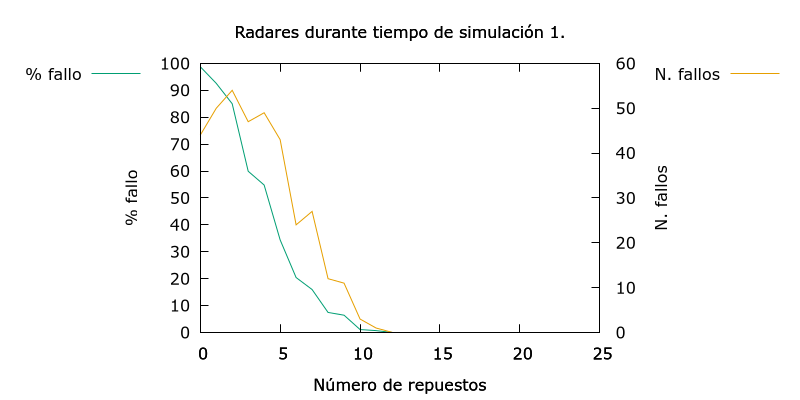
\includegraphics[scale = 0.6]{radares_1.png}
	\caption{Número de fallos y porcentaje de tiempo de fallo en función del número de repuestos.}
	\label{fig:ej4}
\end{figure}

\begin{figure}[H]
	\centering
	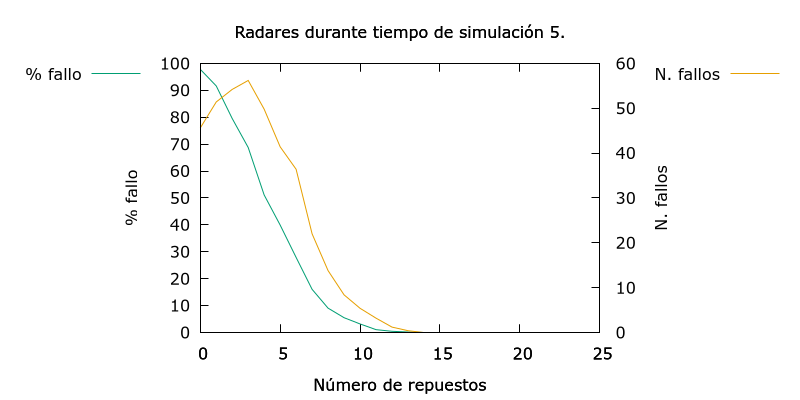
\includegraphics[scale = 0.6]{radares_5.png}
	\caption{Media de la distancia al objetivo respecto al punto de partida con una probabilidad del 25\% de que el sitio este ocupado..}
	\label{fig:ej4}
\end{figure}

\begin{figure}[H]
	\centering
	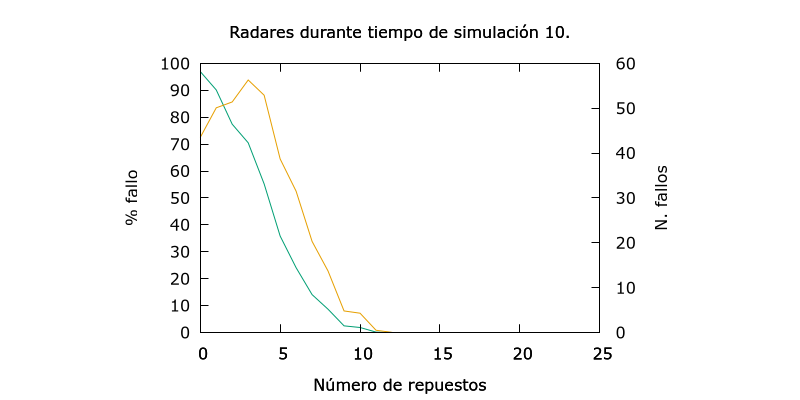
\includegraphics[scale = 0.6]{radares_10.png}
	\caption{Número de fallos y porcentaje de tiempo de fallo en función del número de repuestos.}
	\label{fig:ej4}
\end{figure}

\begin{figure}[H]
	\centering
	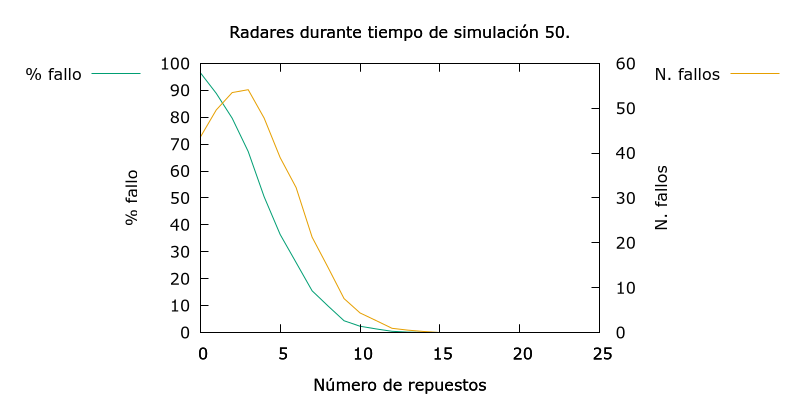
\includegraphics[scale = 0.6]{radares_50.png}
	\caption{Número de fallos y porcentaje de tiempo de fallo en función del número de repuestos.}
	\label{fig:ej4}
\end{figure}

\begin{figure}[H]
	\centering
	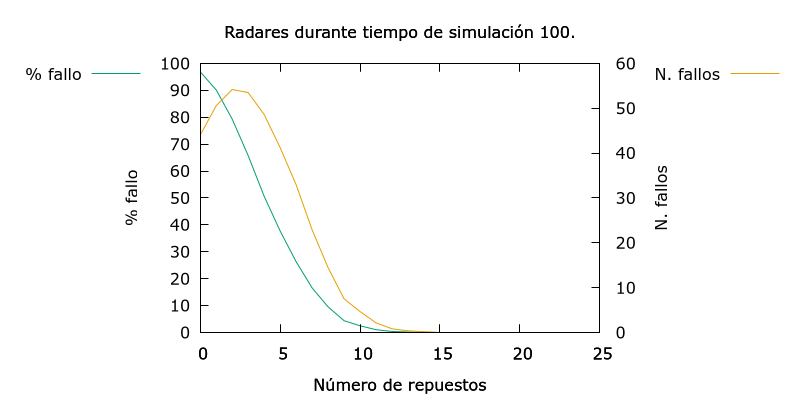
\includegraphics[scale = 0.6]{radares_100.png}
	\caption{Número de fallos y porcentaje de tiempo de fallo en función del número de repuestos.}
	\label{fig:ej4}
\end{figure}

\begin{figure}[H]
	\centering
	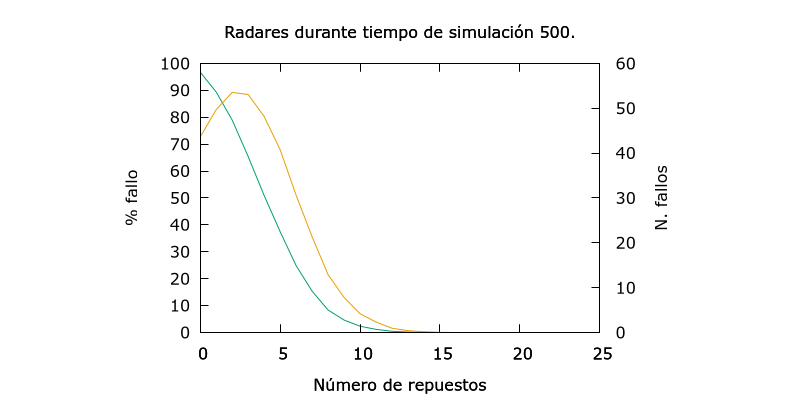
\includegraphics[scale = 0.6]{radares_500.png}
	\caption{Número de fallos y porcentaje de tiempo de fallo en función del número de repuestos.}
	\label{fig:ej4}
\end{figure}

\begin{figure}[H]
	\centering
	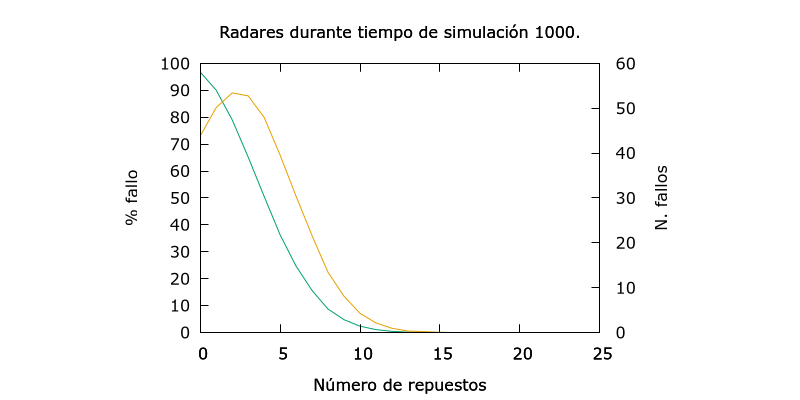
\includegraphics[scale = 0.6]{radares_1000.png}
	\caption{Número de fallos y porcentaje de tiempo de fallo en función del número de repuestos.}
	\label{fig:ej4}
\end{figure}


En principio estas gráficas pueden ser confusas en su primer valor, sin repuestos, ya que aunque tenemos un 100\% de fallo obtenemos menor número de fallos, pero esto es debido a que todas los radares están fallando, obteniendo el 100\% de fallo, y el número de fallos no puede subir ya que no los radares no pueden volver a fallar si todavía no han sido reparados.

Con respecto al número mínimo de repuestos, aunque en las gráficas no se llega a apreciar, en los resultados observamos que cuanto mayor se va haciendo el tiempo de simulación son necesarios más repuestos para tener menos de un 1\% de tiempo de fallo, aunque es cierto que como muestran las gráficas, a partir de 13 o 14 repuestos es despreciable ya que se trata de valores menores al 1\% del tiempo.


\subsection{Influencia del tiempo de fallo de la pieza.}

En este caso estudiaremos la influencia del tiempo de fallo de la pieza en el sistema, es decir, que pasaría si hacemos que la pieza tarde más (o menos) en fallar, manteniendo los tiempos de reparación. Este experimento también nos servirá para evaluar la fiabilidad del sistema, ya que lo normal sería que si mantenemos los tiempos de reparación, si la pieza falla más necesitemos más repuestos, y si falla menos, necesitaremos menos repuestos.

Para este experimento usaré de tiempo de simulación 500, ya que como hemos visto la diferencia entre usar 100, 500 y 1000 apenas es notable.


\begin{figure}[H]
	\centering
	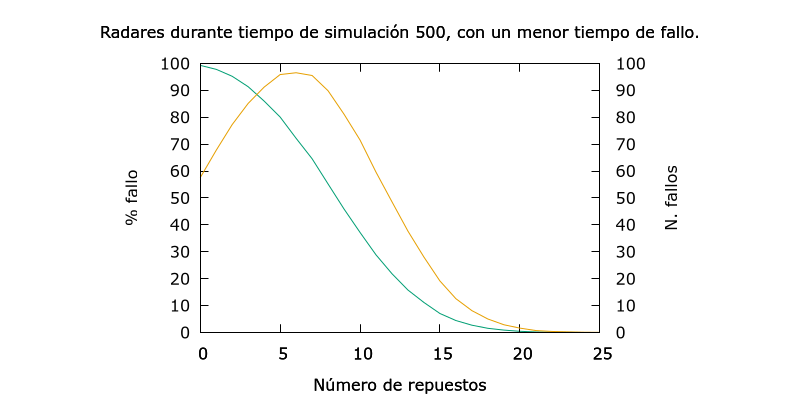
\includegraphics[scale = 0.6]{radares_500_10.png}
	\caption{Número de fallos y porcentaje de tiempo de fallo en función del número de repuestos con un tiempo de fallo de 10 días.}
	\label{fig:ej4}
\end{figure}

\begin{figure}[H]
	\centering
	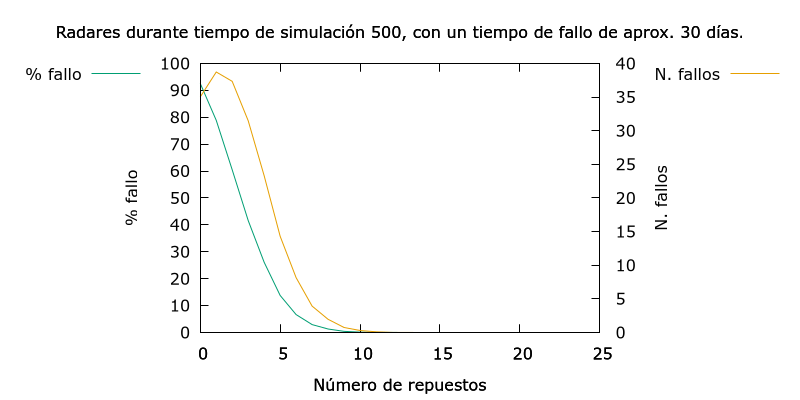
\includegraphics[scale = 0.6]{radares_500_30.png}
	\caption{Número de fallos y porcentaje de tiempo de fallo en función del número de repuestos con un tiempo de fallo de 30 días.}
	\label{fig:ej4}
\end{figure}

Vemos como estos resultados concuerdan y tienen sentido en el sistema, ya que, si los fallos se producen con más frecuencia es necesario tener más repuestos, mientras que con una menor frecuencia de fallos podemos permitirnos tener menos repuestos, siendo necesarios 22 repuestos en el caso en el que los fallos son más frecuentes y 10 repuestos en el caso de los fallos menos frecuentes.


\newpage

\section{Modelo de simulación continuo.}

Para este apartado se nos encarga estudiar un sistema que simula el comportamiento e interacción de dos tipos de peces en un lago, una especie la llamaremos pequeños y a la otra grandes. En dicho lago, debido a las condiciones de tamaño, comida, etc, el número máximo de 10000000 peces pequeños y 36000 peces grandes. Otro detalle a tener en cuenta es que los peces pequeños son hervívoros, no necesitan comida extra además de la que se encuentra en el entorno del lago, mientras que los peces grandes son carnívoros y se alimentan de los peces pequeños.

\subsection{Estudio del sistema para encontrar un equilibrio entre las especies.}

En esta simulación trataremos de encontrar un equilibrio entre peces pequeños y peces grandes que permita a ambas especies sobrevivir.

Tras realizar la simulación durante 10 años (3650 días), con todas las combinaciones de los siguientes valores iniciales:

\begin{itemize}
	\item Peces pequeños: 100, 500, 1000, 1500, 3000, 6000, 10000 y 20000.
	\item Peces grandes: 10, 50, 100, 500, 1000 y 1500.
\end{itemize}

Encontramos tres posibles casos, dos de ellos muy parecidos:

\begin{enumerate}
	\item Los peces grandes devoran toda la población de peces pequeños, y al quedarse sin comida estos tambien mueren.
	\item Se equilibran las poblaciones, el gran número de peces pequeños permite que la población de peces grandes se mantenga, y ese número de peces grandes permite a la especie de peces pequeños reproducirse lo suficiente para evitar extinguirse.
\end{enumerate}


Como vemos, en el primer caso dos ambas especies acaban extintas, mientras que en el segundo caso sobreviven, algunas gráficas de este comportamiento son las siguientes:


\begin{figure}[H]
	\centering
	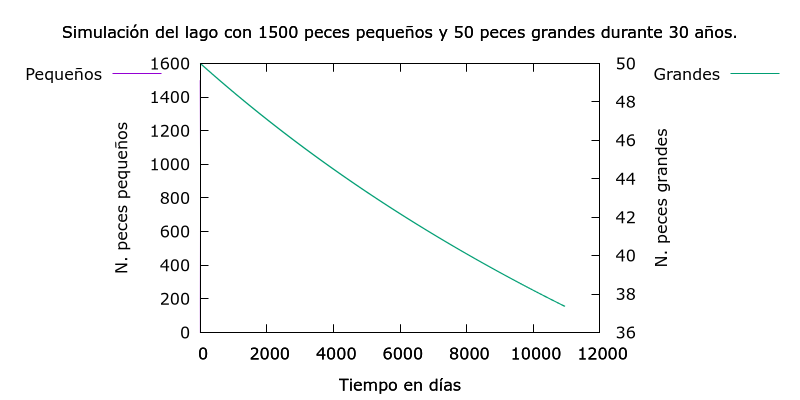
\includegraphics[scale = 0.6]{lago_10950_1500_50.png}
	\caption{Simulación del lago con 1500 peces pequeños y 50 peces grandes.}
	\label{fig:ej4}
\end{figure}

\begin{figure}[H]
	\centering
	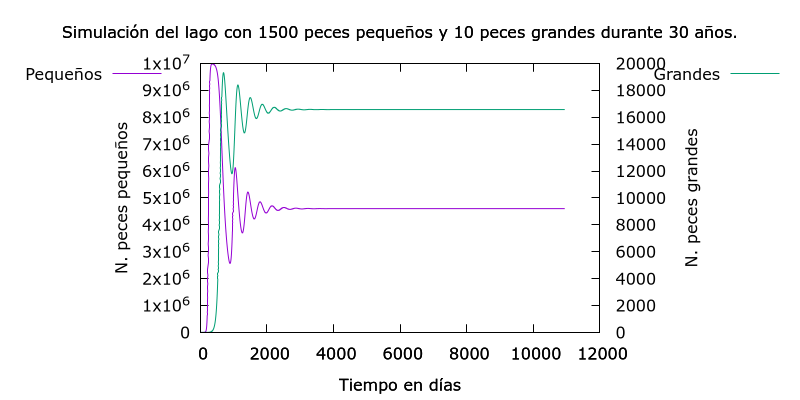
\includegraphics[scale = 0.6]{lago_10950_1500_10.png}
	\caption{Simulación del lago con 1500 peces pequeños y 10 peces grandes.}
	\label{fig:ej4}
\end{figure}

Comentar también que se llega a conseguir este punto de equilibrio cuando comenzamos tan pocos peces grandes que los peces pequeños pueden llegar a su máximo, ya que esta es la única forma que con todas las otras combinaciones se ha llegado a estabilizar el sistema, esto es importante, ya que también influye el número de ejemplares iniciales de cada especie, con 1500 pequeños la única forma de alcanzar la estabilidad es con 10 peces grandes, mientras que con 20000 peces pequeños podemos llegar a tener inicialmente 100 peces grandes.

Otra cosa que podemos observar es como avanzan el número de peces pequeños en función del número de peces grandes:


\begin{figure}[H]
	\centering
	\includegraphics[scale = 0.6]{lago_10950_1500_10_peces.png}
	\caption{Simulación del lago con 1500 peces pequeños y 10 peces grandes.}
	\label{fig:ej4}
\end{figure}

Con esta gráfica comprobamos que el funcionamiento del sistema es correcta, vemos como cuando existe un gran número de peces pequeños, el número de peces grandes crece muy rápido mientras que el número de pequeños disminuye, hasta un punto en el que hay pocos pequeños, y los peces grandes comienzan a bajar, haciendo que tras bajar considerablemente, los peces pequeños comiencen a ser capaces de volver a recuperar población, y así repitiendose el ciclo y estabilizandose en el centro de la espiral.

Tras esta simulación podemos asegurar que hay una configuración que con ese número de ejemplares de cada especie ambas poblaciones se estabilizan y conviven, luego podemos seguir la investigación de si es viable realizar campañas de pesca.


\newpage

\subsection{Estudio de campañas de pesca.}

Aunque existen varios valores con los que se estabilizan las poblaciones, de ahora en adelante utilizaré 1500 peces pequeños y 10 grandes, ya que una vez se estabiliza el sistema es indiferente.


Para estudiar las posibles campañas de pesca he lanzado la simulación con todas las siguientes combinaciones:

\begin{itemize}
	\item Periodo entre cada pesca: 90, 180, 365, 750, 1400, 2000 y 5000 días.
	\item Porcentaje de peces grandes pescados: 10, 30, 50, 70 y 90\% de los peces.
\end{itemize}

De estas combinaciones todas funcionan, ya la disminución de los peces grandes permite que los pequeños crezcan de forma muy rápida, y al no llegar a matar a todos los peces grandes, los restantes, con la comida extra, consiguen recuperarse rápidamente. Si es cierto que llegamos a observar varios escenarios, donde el número de peces es muy bajo, o muy inestable, pero siempre se llega a estabilizar, aunque sea en números muy muy bajos, sin llegar a desaparecer.

Algunos ejemplos de los distintos casos:



\begin{figure}[H]
	\centering
	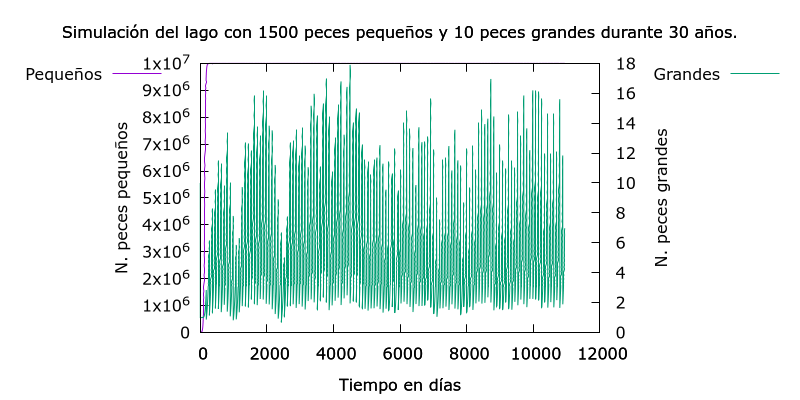
\includegraphics[scale = 0.6]{lago_10950_1500_10_0.90_90.png}
	\caption{Pescas cada 90 días, del 10\% de los peces grandes.}
	\label{fig:ej4}
\end{figure}

\begin{figure}[H]
	\centering
	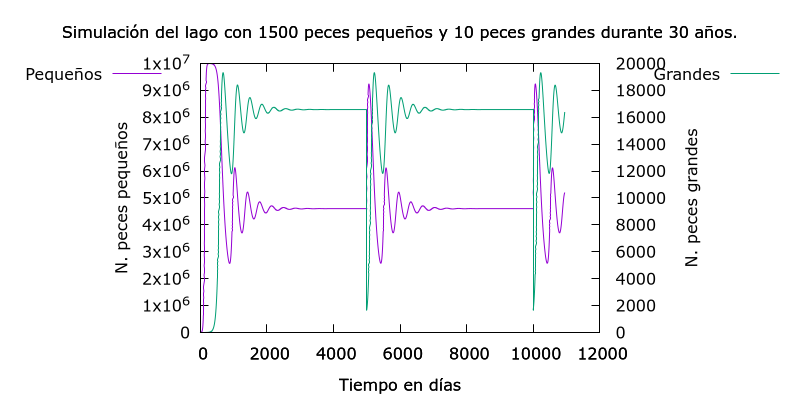
\includegraphics[scale = 0.6]{lago_10950_1500_10_0.90_5000.png}
	\caption{Pescas cada 5000 días, del 10\% de los peces grandes.}
	\label{fig:ej4}
\end{figure}

En la primera gráfica podemos ver que con tiempos de pesca tan seguidos, los peces pequeños se mantienen en su límite superior de población, sin embargo el máximo de peces grandes no supera los 20, mientras que en la segunda gráfica, al hacer pescas tan separadas en el tiempo si nos permite que la población de peces grandes sea mucho mayor y las pescas más grandes.

Como vemos, el principal problema que encontramos en estas gráficas es que el tiempo entre pescas es demasiado pequeño no permitiendo explotar más, o demasiado alto y hay periodos en los que podriamos conseguir mejores pescas.

A continuación muestro la gráfica de todas las combinaciones y como avanza la cantidad de pesca:


\begin{figure}[H]
	\centering
	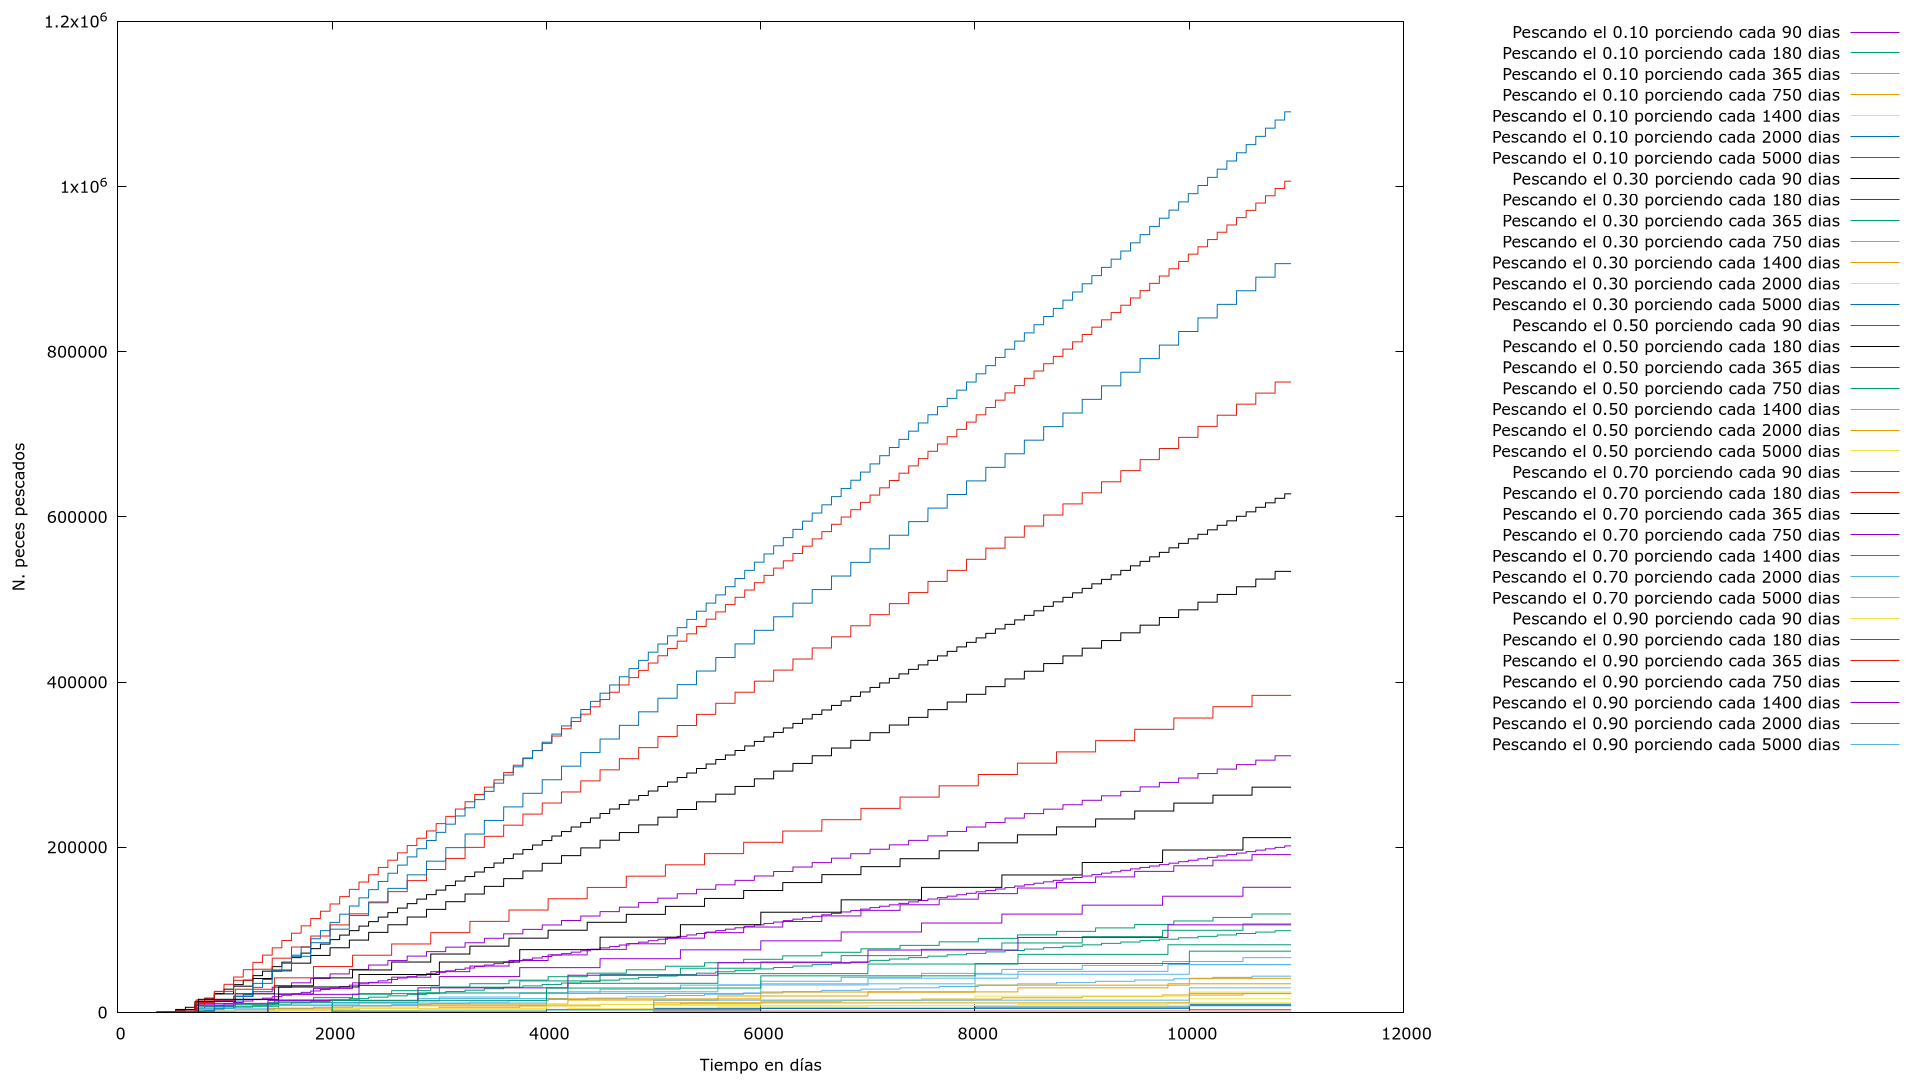
\includegraphics[scale = 0.25]{total.png}
	\caption{Recolección de cada forma de pesca.}
	\label{fig:ej4}
\end{figure}


Como vemos en la gráfica, debido a la gran cantidad de simulaciones realizadas, no somos capaces de distinguir la mejor, sin embargo vemos que las mejores se realizan en periodos cortos de tiempo:


\begin{figure}[H]
	\centering
	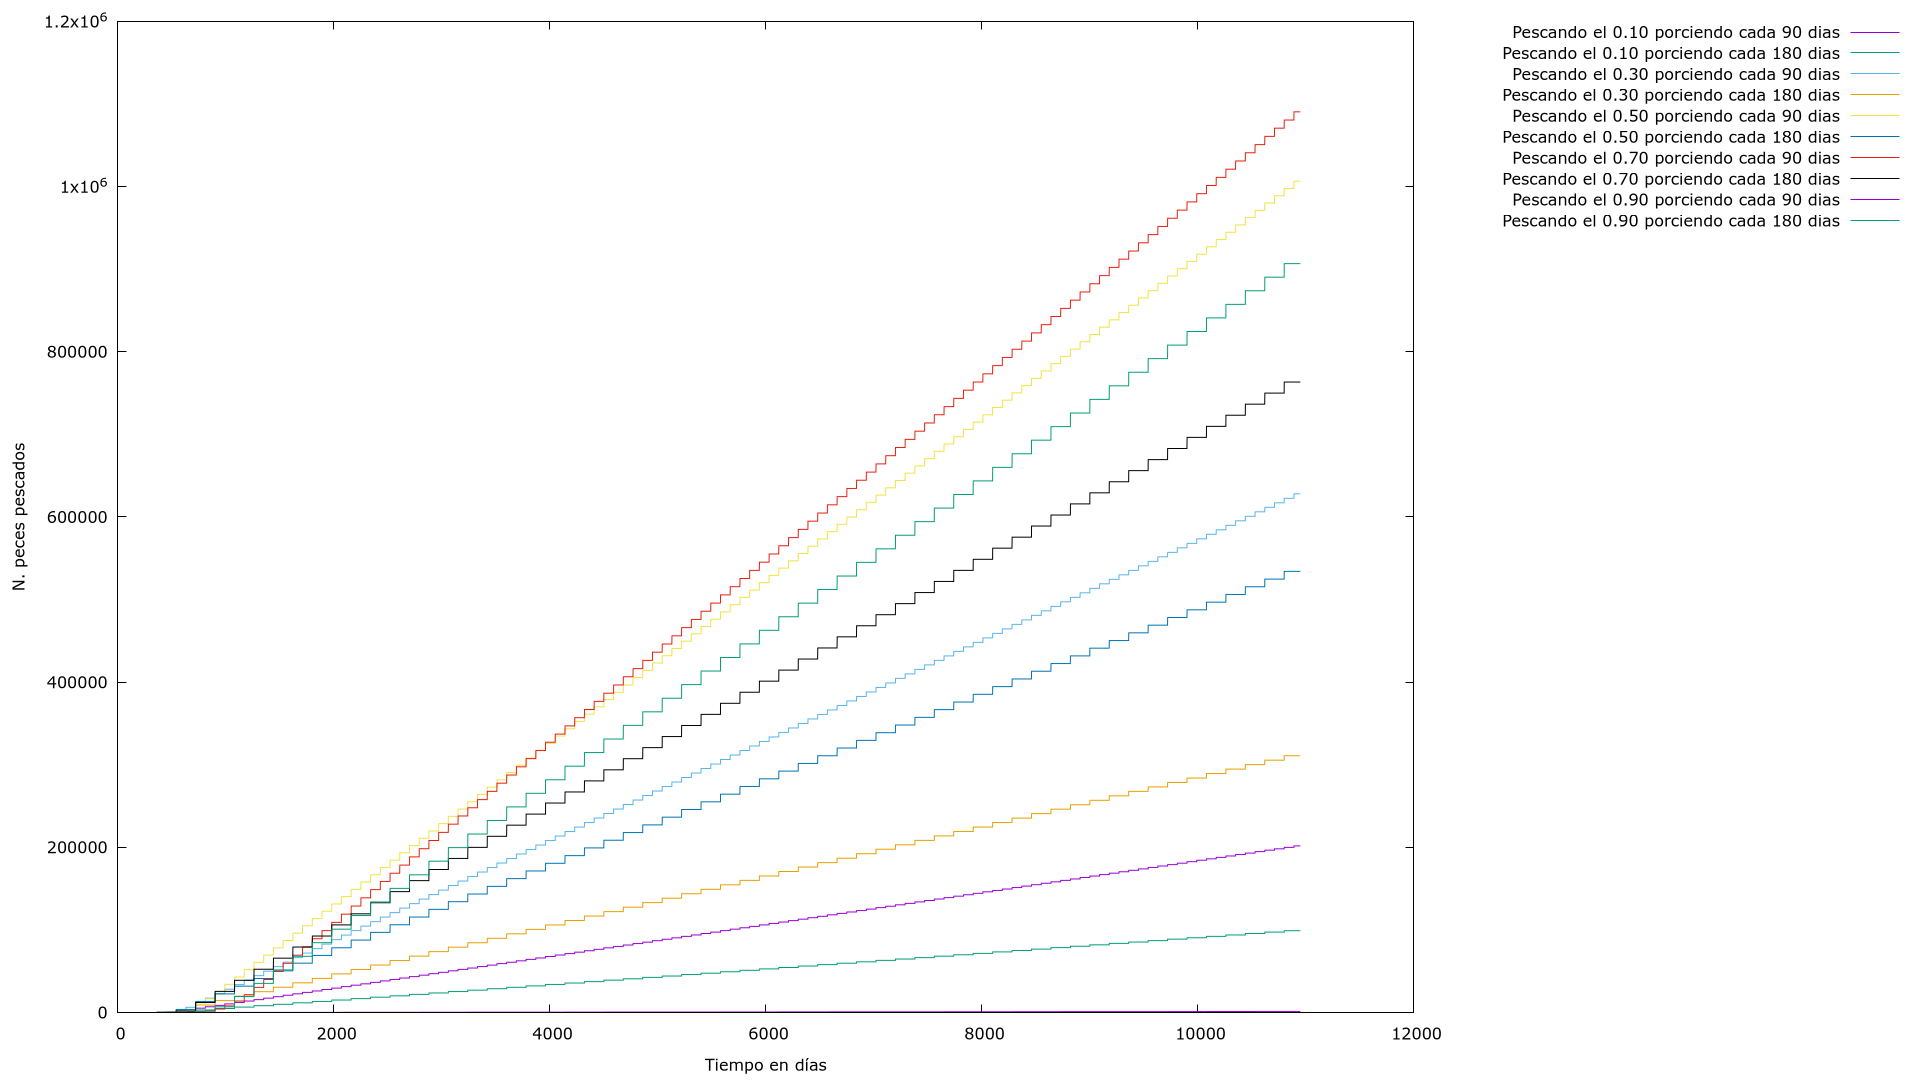
\includegraphics[scale = 0.25]{total_reducido.png}
	\caption{Recolección de cada forma de pesca.}
	\label{fig:ej4}
\end{figure}


Como podemos ver en esta gráfica, vemos como la mejor forma de pesca es pescando el 70\% de los peces grandes cada 90 días:


\begin{figure}[H]
	\centering
	\includegraphics[scale = 0.6]{lago_10950_1500_10_0.70_90.png}
	\caption{Pescas cada 90 días, del 70\% de los peces grandes.}
	\label{fig:ej4}
\end{figure}

En esta gráfica podemos observar prefectamente como con esta forma de pesca los peces grandes son capaces de recuperarse a niveles muy altos (unos 14000) antes de la próxima pesca, incluso pescando un nivel tan alto como el 70\%, permitiendo la máxima producción.


\begin{figure}[H]
	\centering
	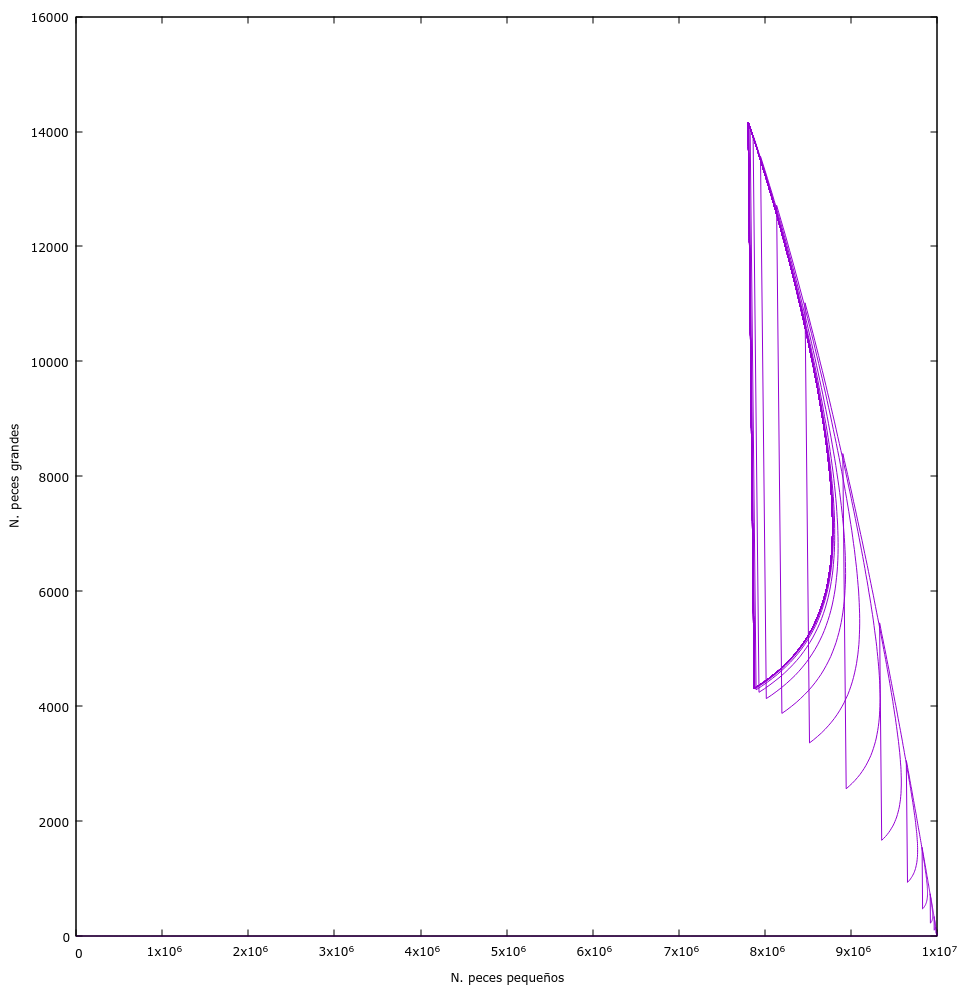
\includegraphics[scale = 0.6]{pesca_ratio.png}
	\caption{Relación de peces pequeños y grandes en el mejor caso de pescas.}
	\label{fig:ej4}
\end{figure}

También podemos observar como la relación entre los peces se mantiene en una linea a causa de las pescas, pero manteniendose en el mismo sitio, lo que nos permitiría seguir con este ritmo de pesca manteniendo las relaciones de peces.

% \begin{thebibliography}{9}
%
%
% \end{thebibliography}

\end{document}
